
\documentclass[11pt,a4paper]{article}
\usepackage[utf8]{inputenc}
\usepackage[T1]{fontenc}
\usepackage[spanish,es-nodecimaldot]{babel}
\usepackage[a4paper,left=1.7cm,right=1.7cm,top=20mm,bottom=20mm]{geometry}
\usepackage{amsmath,amssymb,amsfonts,mathtools,bm}
\usepackage{braket}
\usepackage{graphicx}
\usepackage{float}
\usepackage{booktabs}
\usepackage{enumitem}
\usepackage{xcolor}
\usepackage{lmodern,microtype}
\usepackage{fancyhdr}
\usepackage{titlesec}
\usepackage[colorlinks=true,linkcolor=black,urlcolor=black,citecolor=black]{hyperref}
\numberwithin{equation}{section}
\renewcommand{\boxed}[1]{#1}
\setlength{\parindent}{0pt}
\setlength{\parskip}{5pt}
\newcommand{\dd}{\,\mathrm d}
\newcommand{\ii}{\mathrm i}
\newcommand{\e}{\mathrm e}
\newcommand{\hb}{\hbar}
\newcommand{\R}{\mathbb R}
\newcommand{\C}{\mathbb C}
\newcommand{\id}{\mathbb I}

\pagestyle{fancy}
\setlength{\headheight}{14pt}
\fancyhf{}
\fancyhead[L]{\textit{Tarea 12}}
\fancyhead[R]{Mecánica Cuántica I}
\begin{document}
\begin{titlepage}
\centering
\vspace*{1.8cm}

\includegraphics[width=.22\textwidth]{UdeC_escudo.png}
\vspace{1.1cm}
{\Huge\bfseries Tarea 12\par}
\vspace{.4cm}
{\Huge\bfseries Mecánica Cuántica I\par}
\vspace{1.5cm}
{\Large José Ignacio Rosas Sepúlveda\par}
\vspace{.8cm}
{\Large Solución\par}
\vfill
\thispagestyle{empty}
\end{titlepage}
\tableofcontents
\newpage
\section*{Enunciado}
\addcontentsline{toc}{section}{Enunciado}
\begin{enumerate}[label=\arabic*.-]
\item Una partícula de spin $1/2$ interactúa con un campo magnético uniforme $B_z\hat z$. Su Hamiltoniano es
\begin{equation}
H=-\gamma B_zS_z=-\frac{\gamma\hbar B_z}{2}\sigma_z,
\end{equation}
donde $\gamma$ es la constante giromagnética. Inicialmente
\begin{equation}
\ket{\psi(0)}=\ket{+x}=\frac{1}{\sqrt2}(\ket\uparrow+\ket\downarrow).
\end{equation}
\begin{enumerate}[label=\alph*)]
\item Encuentre $U(t)$.
\item Encuentre $\ket{\psi(t)}$.
\item Calcule la probabilidad de proyectar sobre $\ket\uparrow$.
\item Calcule la probabilidad de proyectar sobre $\ket\downarrow$.
\item Calcule la probabilidad de proyectar sobre $\ket{+x}$.
\item Calcule la probabilidad de proyectar sobre $\ket{-x}$.
\item Calcule $\langle\sigma_x\rangle$ y $\Delta\sigma_x$.
\item Grafique ambas cantidades como funciones de $\tau=\gamma B_zt$.
\item Calcule $\langle\sigma_z\rangle$ y $\Delta\sigma_z$.
\item Calcule $\langle\sigma_y\rangle$ y $\Delta\sigma_y$.
\item Grafique estas últimas como funciones de $\tau$.
\end{enumerate}
\item Para una partícula en caída libre,
\begin{equation}H=\frac{P^2}{2m}+mgX.\end{equation}
Usando el cuadro de Heisenberg:
\begin{enumerate}[label=\alph*)]
\item encuentre $\langle P(t)\rangle$ y $\Delta P(t)$;
\item encuentre $\langle X(t)\rangle$ y $\Delta X(t)$.
\end{enumerate}
\end{enumerate}


\section{Problema 1}
El Hamiltoniano es
\begin{equation}
H=-\gamma B_zS_z=-\frac{\hb\Omega}{2}\sigma_z,
\qquad \Omega=\gamma B_z.
\end{equation}
Como $\sigma_z^2=\id$,
\begin{equation}
\boxed{U(t)=\e^{-\ii Ht/\hb}
=\cos\frac{\Omega t}{2}\,\id+\ii\sin\frac{\Omega t}{2}\,\sigma_z.}
\end{equation}
En la base $\{\ket\uparrow,\ket\downarrow\}$,
\begin{equation}
U(t)=\begin{pmatrix}\e^{\ii\Omega t/2}&0\\0&\e^{-\ii\Omega t/2}\end{pmatrix}.
\end{equation}
Para $\ket{\psi(0)}=\ket{+x}=(\ket\uparrow+\ket\downarrow)/\sqrt2$,
\begin{equation}
\boxed{\ket{\psi(t)}=\frac1{\sqrt2}
\left(\e^{\ii\Omega t/2}\ket\uparrow+\e^{-\ii\Omega t/2}\ket\downarrow\right).}
\end{equation}

\subsection{Probabilidades de medición}
En la base de $S_z$ las amplitudes tienen módulo $1/\sqrt2$:
\begin{equation}
\boxed{P(\uparrow_z)=P(\downarrow_z)=\frac12.}
\end{equation}
En la base de $S_x$,
\begin{equation}
\braket{+x|\psi(t)}=\cos\frac{\Omega t}{2},\qquad
\braket{-x|\psi(t)}=\ii\sin\frac{\Omega t}{2},
\end{equation}
por lo que
\begin{equation}
\boxed{P(+x)=\cos^2\frac{\Omega t}{2},\qquad
P(-x)=\sin^2\frac{\Omega t}{2}.}
\end{equation}

\subsection{Promedios y dispersiones de Pauli}
Con $\tau=\Omega t$,
\begin{align}
\langle\sigma_x\rangle&=\cos\tau,&
\Delta\sigma_x&=|\sin\tau|,\\
\langle\sigma_y\rangle&=-\sin\tau,&
\Delta\sigma_y&=|\cos\tau|,\\
\langle\sigma_z\rangle&=0,&
\Delta\sigma_z&=1.
\end{align}
Se usó $\sigma_i^2=\id$. Las correspondientes cantidades de spin se obtienen multiplicando por $\hb/2$.
\begin{figure}[H]\centering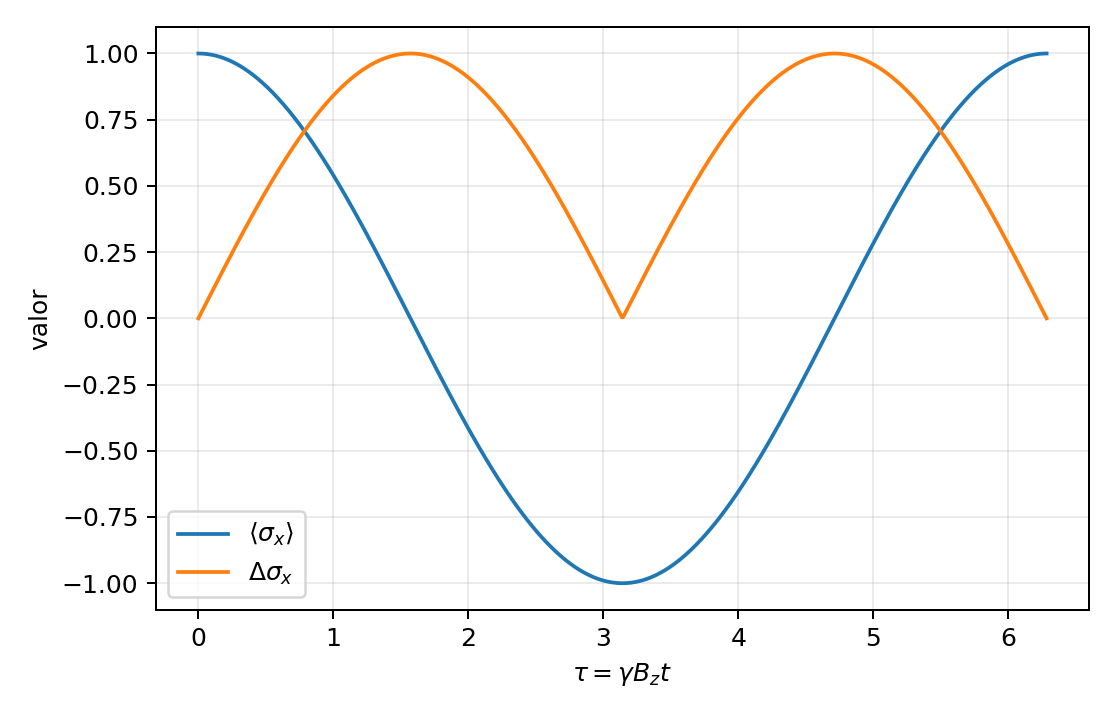
\includegraphics[width=.67\textwidth]{figures/sigma_x.png}\caption{Promedio y desviación de $\sigma_x$.}\end{figure}
\begin{figure}[H]\centering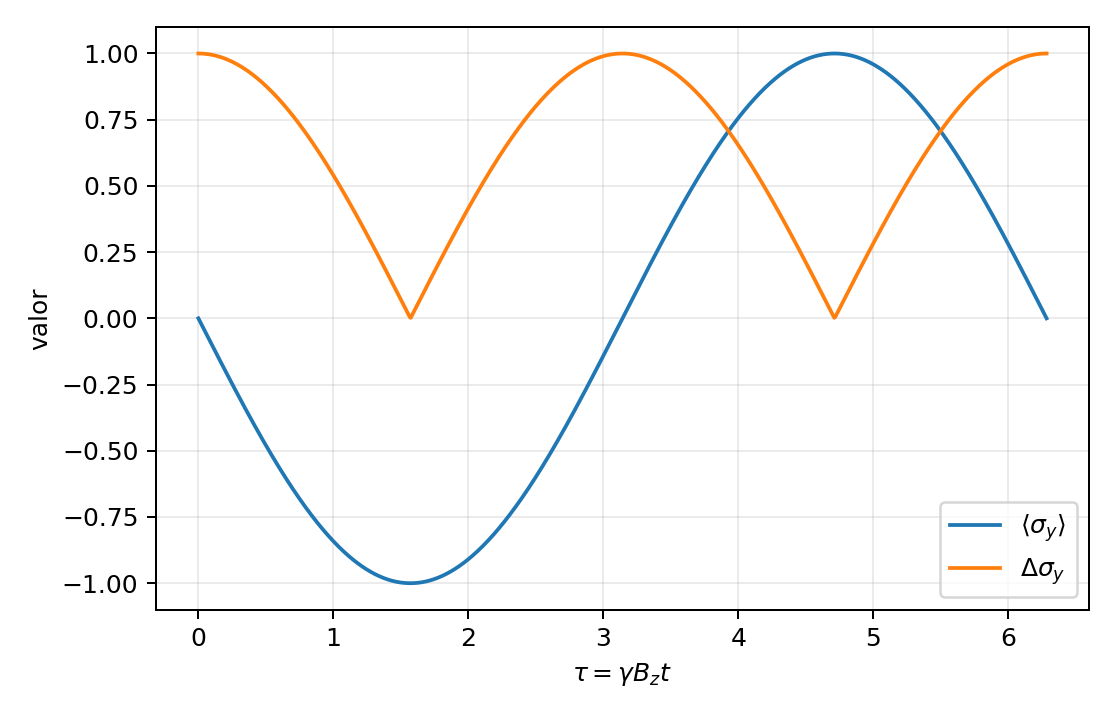
\includegraphics[width=.67\textwidth]{figures/sigma_y.png}\caption{Promedio y desviación de $\sigma_y$.}\end{figure}

\paragraph{Comentario.}
El vector de Bloch precesa alrededor del eje $z$. La distribución de $S_z$ permanece invariante porque $[H,S_z]=0$, mientras que $S_x$ y $S_y$ oscilan.


\section{Problema 2}
Para
\begin{equation}
H=\frac{P^2}{2m}+mgX,
\end{equation}
las ecuaciones de Heisenberg son
\begin{equation}
\dot P=\frac{\ii}{\hb}[H,P]=-mg,
\qquad
\dot X=\frac{\ii}{\hb}[H,X]=\frac Pm.
\end{equation}
Integrando,
\begin{equation}
\boxed{P(t)=P(0)-mgt,}
\end{equation}
\begin{equation}
\boxed{X(t)=X(0)+\frac{t}{m}P(0)-\frac12gt^2.}
\end{equation}
Por tanto,
\begin{align}
\langle P(t)\rangle&=\langle P(0)\rangle-mgt,&
\Delta P(t)&=\Delta P(0),\\
\langle X(t)\rangle&=\langle X(0)\rangle+\frac tm\langle P(0)\rangle-\frac12gt^2.
\end{align}
La dispersión espacial requiere conservar la covarianza inicial:
\begin{equation}
\boxed{
(\Delta X(t))^2=(\Delta X_0)^2+\frac{t^2}{m^2}(\Delta P_0)^2
+\frac{t}{m}\left\langle\{\Delta X_0,\Delta P_0\}\right\rangle.}
\end{equation}

\paragraph{Hipótesis necesaria.}
No es legítimo eliminar el término de covarianza sin especificar el estado inicial. Sólo para estados con covarianza simetrizada nula se reduce a $(\Delta X_0)^2+t^2(\Delta P_0)^2/m^2$.



\end{document}
